\documentclass[10pt,twocolumn]{IEEEtran}

\usepackage{times}
\usepackage[T1]{fontenc}
\usepackage[utf8]{inputenc}
\usepackage{microtype}
\usepackage{array}
\usepackage{graphicx}
\usepackage{cuted}
\usepackage{tikz}
\usetikzlibrary{arrows.meta,positioning}
\usepackage[hidelinks]{hyperref}
\usepackage[backend=biber,style=ieee,doi=true,url=true,isbn=false,hyperref=false,
            maxbibnames=1,minbibnames=1]{biblatex}
\addbibresource{references.bib}

% Use label colons instead of the long dashes generated by IEEEtran.
\makeatletter
\def\abstract{\normalfont
    \if@twocolumn
      \@IEEEabskeysecsize\bfseries\textit{\abstractname}:\enspace\relax
    \else
      \bgroup\par\addvspace{0.5\baselineskip}\centering\vspace{-1.78ex}
      \@IEEEabskeysecsize\textbf{\abstractname}\par
      \addvspace{0.5\baselineskip}\egroup\quotation\@IEEEabskeysecsize
    \fi\@IEEEgobbleleadPARNLSP}
\def\IEEEkeywords{\normalfont
    \if@twocolumn
      \@IEEEabskeysecsize\bfseries\textit{\IEEEkeywordsname}:\enspace\relax
    \else
      \bgroup\par\addvspace{0.5\baselineskip}\centering
      \@IEEEabskeysecsize\textbf{\IEEEkeywordsname}\par
      \addvspace{0.5\baselineskip}\egroup\quotation\@IEEEabskeysecsize
    \fi\@IEEEgobbleleadPARNLSP}
\makeatother

\title{Evidence-Bounded Visual Multimodal Privacy Protection for
Egocentric Personal Images}

\author{
\begin{tabular}{@{}>{\centering\arraybackslash}p{0.46\textwidth}>{\centering\arraybackslash}p{0.46\textwidth}@{}}
\textbf{Arun Narayanan} & \textbf{Vaseekaran Krishnan Vinodhan} \\
A00048672 & A00050240 \\
\footnotesize arun.narayanan2@mail.dcu.ie &
\footnotesize vaseekaran.krishnanvinodhan2@mail.dcu.ie \\
\multicolumn{2}{c}{School of Computing, Dublin City University (AI)} \\
\multicolumn{2}{c}{Dublin, Ireland} \\
\end{tabular}
\vspace{0.2\baselineskip}
}

\IEEEspecialpapernotice{Supervised by Dr.~Liting Zhou, School of Computing,
Dublin City University.}

\begin{document}

\maketitle

\begin{abstract}
Egocentric personal images may expose faces, readable text, and screens within
the same frame, but privacy methods are often evaluated as separate tasks. This
paper presents an evidence-bounded visual multimodal framework that combines
detection, protection, evaluation, and objective-aware routing. Experiments use
frozen, manually reviewed protocols derived from CASTLE. Combined-risk presence
detection reached 0.9804 recall on the held-out multimodal split, although
localisation errors and residual text readability remained. Face anonymisation
experiments also showed that no evaluated method was uniformly best across
objectives and conditions. The Objective-Aware Privacy Router (OAPR) therefore
selects only methods that satisfy privacy, utility, visual-safety, runtime, and
failure constraints, with deterministic fallbacks where required. The framework
supports reproducible privacy-risk reduction for egocentric image sharing, but
does not claim complete anonymisation, complete semantic privacy, or production
readiness.
\end{abstract}

\begin{IEEEkeywords}
Egocentric vision, personal image privacy, visual multimodal privacy, face
anonymisation, text and screen redaction, objective-aware routing.
\end{IEEEkeywords}

\section{Introduction}
\label{sec:introduction}

\subsection{Privacy Risk in Egocentric Images}

Wearable and first-person cameras capture useful records of activities,
surroundings, and interactions. They also collect information outside the
wearer's intended subject. One image may contain a bystander's face, personal
text, and content displayed on a phone or computer screen. CASTLE illustrates
the scale and diversity of current egocentric collections~\cite{rossetto2025castle}.
EgoPrivacy further shows that sensitive personal and situational information can
remain inferable even when a face is unavailable~\cite{li2025egoprivacy}. In
this paper, \emph{visual multimodal privacy} means protecting several privacy
surfaces within the same image, principally faces, text, and screens. It does not
refer to the fusion of different sensor types.

\subsection{Technical and Research Gap}

Egocentric capture makes each privacy surface difficult to process. Faces vary
in size, pose, blur, occlusion, and illumination. Text can be small, oblique, or
only partly readable. Screens introduce reflections, borders, and complex visual
content. Missing a sensitive region leaves direct exposure, but unnecessarily
strong redaction can reduce scene utility. Existing de-identification research
documents this conflict between privacy and utility~\cite{khan2025persondeid},
while egocentric screen detection remains a specialised task~\cite{li2026screen}.
Most studies therefore optimise one component or one method family in isolation.
They do not establish how several protection stages should be evaluated and
combined when their accuracy, reliability, visual quality, and compute costs
differ.

\subsection{Framework and Research Questions}

This work treats privacy protection as an evidence-supported selection problem.
CASTLE provides the evaluation setting, while the research questions address
egocentric images generally. Reviewed protocols compare detectors, deterministic
and generative face protection, joint face, text, and screen processing, and
residual failures. OAPR then applies privacy floors, method eligibility,
visual-safety checks, runtime evidence, and fallbacks before selecting an action.
The study asks:

\begin{enumerate}
\item[\textbf{RQ1}] Which face-detection approaches provide the greatest
robustness on egocentric images under practical compute constraints?
\item[\textbf{RQ2}] How do deterministic and generative face-anonymisation
methods compare in privacy protection, image utility, visual quality, runtime,
and reliability?
\item[\textbf{RQ3}] To what extent can an integrated pipeline jointly detect and
protect faces, readable text, and screens while preserving the utility of
egocentric images?
\item[\textbf{RQ4}] How does adaptive method selection based on image conditions
and privacy objectives compare with using a fixed anonymisation strategy?
\end{enumerate}

\subsection{Contributions}

The paper contributes three connected outcomes. First, it provides reviewed and
separated protocols for detector, anonymisation, and visual multimodal
evaluation. Second, it compares eligible privacy methods using direct metrics
and observed failure behaviour, including visual checks that prevent a high
numerical score from determining deployment alone. Third, it integrates these
findings through OAPR, which records the selected and applied actions and uses a
safe fallback when an advanced action is ineligible or fails. Together, these
outcomes support an auditable pipeline for risk reduction without treating any
single method as universally optimal.

\section{Related Work}
\label{sec:related-work}

\subsection{Egocentric Privacy and De-identification}

Egocentric cameras record first-person activities and context, but can also
expose wearers, bystanders, readable text, screens, and environmental information.
CASTLE provides synchronised wearable and fixed-camera views for multimodal
understanding, creating challenging imagery for privacy evaluation
~\cite{rossetto2025castle}. EgoPrivacy demonstrates that an
egocentric stream can reveal the wearer's identity, demographics, and situation
through cues beyond visible faces~\cite{li2025egoprivacy}. Thapar et al. similarly
show that camera motion can encode wearer identity and that suppressing this cue
must be balanced against activity-recognition utility~\cite{thapar2021anonymizing}.
These works establish that privacy in first-person imagery is contextual as well
as facial. However, the wider de-identification literature remains dominated by
face or person transformation considered separately from text and screens
~\cite{khan2025persondeid}.

\subsection{Detection in Difficult Egocentric Conditions}

Detection research offers complementary design choices. YOLO formulates object
detection as efficient single-network regression~\cite{redmon2016yolo}; DETR
uses global context and direct set prediction~\cite{carion2020detr}; and SCRFD
redistributes samples and computation to improve efficient face detection
~\cite{guo2022scrfd}. Their published benchmarks establish general detection
or unconstrained face-detection performance, not privacy-weighted reliability on
egocentric images. This distinction matters because an undetected face creates
privacy exposure, while excessive false positives remove useful scene content.
Architecture-level results alone therefore do not identify the best operational
policy for this setting.

\subsection{Face Anonymisation}

Classical k-Same de-identification groups similar faces and replaces them with
an averaged representative, providing an interpretable privacy principle but
visibly altering image content~\cite{newton2005deidentifying}. Blur, masking, and related
deterministic transformations remain simple and predictable, although stronger
settings reduce facial and scene utility. Recent generative work seeks a better
balance. FALCO and StyleID manipulate latent representations to suppress identity
while retaining facial attributes~\cite{barattin2023falco,le2023styleid}.
RiDDLE adds a diversified, reversible latent encryptor
~\cite{li2023riddle}. Diffusion approaches pursue detailed synthesis, attribute
preservation, or local control, as illustrated by FAMS, Reverse Personalization,
and NullFace~\cite{kung2025fams,kung2026reverse,kung2026nullface}.

The methods differ in threat model, reversibility, controllability, required
inputs, and evaluation protocol. Their reported results are largely obtained on
face-centred benchmarks rather than challenging egocentric imagery.
Consequently, strong source-paper scores do not establish reliable transfer to
small, blurred, occluded, or non-frontal faces. They also do not capture failed
execution or conspicuous visual artefacts. A common target-domain protocol must
therefore consider numerical privacy and utility together with runtime,
reliability, and direct visual inspection.

\subsection{Text, Screens, and Multimodal Visual Privacy}

Scene-text and screen research addresses privacy surfaces that face-only methods
leave visible. CRAFT detects character regions and associations, supporting the
detection of text with irregular orientations and shapes~\cite{baek2019craft}.
Egocentric screen
detection has also benefited from multiple views and vision-language reasoning
~\cite{li2026screen}. PrivacyLens demonstrates broader on-device removal of
personally identifiable content by combining RGB and thermal sensing
~\cite{iravantchi2024privacylens}. These approaches are valuable but solve
different tasks or assume different sensors. They do not by themselves determine
how face, text, and screen decisions should be combined within a unified
RGB-image privacy policy,
nor how residual readable content should be reported after redaction.

\subsection{Privacy, Utility, and Failure Evaluation}

Face recognition models provide practical attackers for measuring whether
identity remains recoverable. ArcFace supplies discriminative angular-margin
embeddings, AdaFace adapts its margin to image quality, and FaceNet provides an
established metric-learning baseline
~\cite{deng2019arcface,kim2022adaface,schroff2015facenet}. Such attacker
scores measure one privacy channel, not complete protection. Visual utility also
requires more than pixel agreement: SSIM measures structural similarity, whereas
LPIPS uses deep features to better reflect perceptual judgements
~\cite{wang2004ssim,zhang2018lpips}. None of these metrics directly captures
conspicuous synthesis artefacts, altered gaze or pose, false-positive
anonymisation, or residual readable text. This motivates an evaluation that keeps
privacy, utility, localisation, runtime, execution failure, and visual safety as
distinct evidence before any method is promoted.

\subsection{Research Gap and Positioning}

Across the reviewed literature, privacy-weighted face detection, joint face,
text, and screen protection, comparable privacy, utility, runtime, and failure
evaluation, direct visual review, and gated method selection are not evaluated
together under one reviewed egocentric protocol. This work addresses that
integration gap by evaluating selected components under shared protocols and
connecting their evidence to method eligibility and fallback decisions. The
framework remains bounded to the stated protocols and does not claim complete
privacy or universal superiority.

\section{Methodology}
\label{sec:methodology}

\subsection{Research Design and Evidence Boundaries}

The methodology follows the four research questions through separate reviewed
protocols for face detection, face anonymisation, and visual multimodal privacy.
Development decisions are separated from held-out evaluation, and every promoted
policy is linked to its source metrics, failure evidence, and applied outputs.
CASTLE provides the source imagery from which the reviewed experimental protocols
are constructed, while conclusions are bounded to the tested protocols and
evaluated implementations. The following subsections define the data surfaces,
protocol construction, evaluation boundaries and sequence, and method-selection
procedure.

\begin{figure*}[!t]
\centering
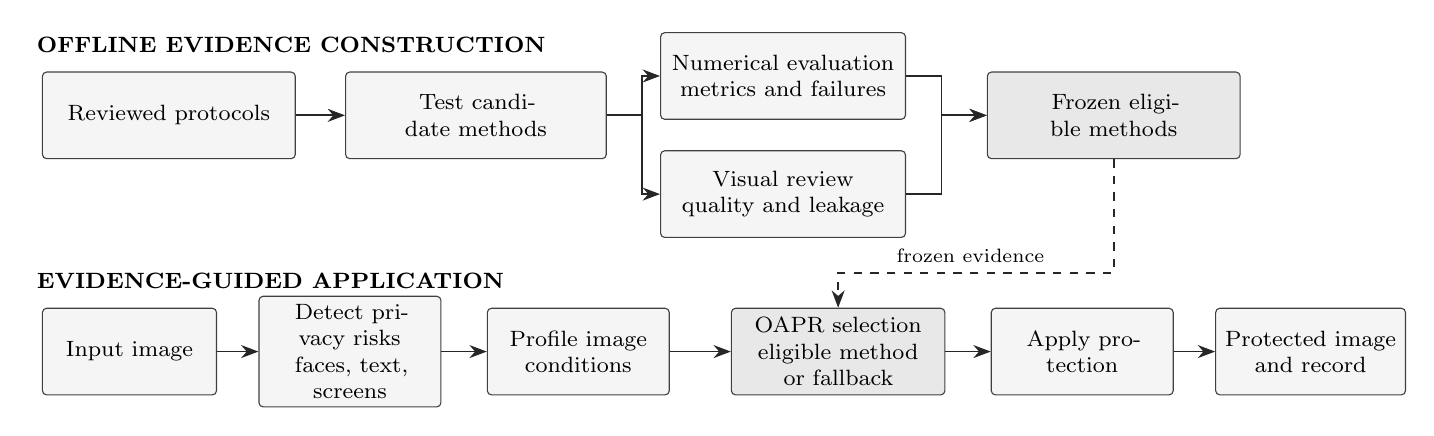
\begin{tikzpicture}[
  x=1cm,y=1cm,
  stage/.style={draw=black!75, rounded corners=1.5pt, fill=black!4,
    minimum height=11mm, align=center, inner xsep=3pt, inner ysep=3pt,
    font=\footnotesize},
  evidence/.style={stage, fill=black!9},
  path/.style={-{Stealth[length=2.2mm]}, line width=0.65pt, draw=black!85},
  evidencepath/.style={path, dashed}
]
\node[font=\footnotesize\bfseries, anchor=west] at (-0.1,3.65)
  {OFFLINE EVIDENCE CONSTRUCTION};
\node[stage, text width=3.0cm] (protocol) at (1.7,2.75)
  {Reviewed protocols};
\node[stage, text width=3.1cm] (candidates) at (5.6,2.75)
  {Test candidate methods};
\node[stage, text width=2.9cm] (quant) at (9.5,3.25)
  {Numerical evaluation\\metrics and failures};
\node[stage, text width=2.9cm] (visual) at (9.5,1.75)
  {Visual review\\quality and leakage};
\node[evidence, text width=3.0cm] (frozen) at (13.7,2.75)
  {Frozen eligible methods};
\draw[path] (protocol) -- (candidates);
\draw[path] (candidates.east) -- ++(0.45,0) |- (quant.west);
\draw[path] (candidates.east) -- ++(0.45,0) |- (visual.west);
\draw[path] (quant.east) -- ++(0.45,0) |- (frozen.west);
\draw[path] (visual.east) -- ++(0.45,0) |- (frozen.west);

\node[font=\footnotesize\bfseries, anchor=west] at (-0.1,0.65)
  {EVIDENCE-GUIDED APPLICATION};
\node[stage, text width=2.0cm] (input) at (1.2,-0.25)
  {Input image};
\node[stage, text width=2.1cm] (detect) at (4.0,-0.25)
  {Detect privacy risks\\faces, text, screens};
\node[stage, text width=2.1cm] (profile) at (6.9,-0.25)
  {Profile image conditions};
\node[evidence, text width=2.5cm] (oapr) at (10.2,-0.25)
  {OAPR selection\\eligible method or fallback};
\node[stage, text width=2.1cm] (apply) at (13.3,-0.25)
  {Apply protection};
\node[stage, text width=2.2cm] (output) at (16.2,-0.25)
  {Protected image and record};
\draw[path] (input) -- (detect);
\draw[path] (detect) -- (profile);
\draw[path] (profile) -- (oapr);
\draw[path] (oapr) -- (apply);
\draw[path] (apply) -- (output);
\coordinate (evidencebend) at (10.2,0.75);
\draw[evidencepath] (frozen.south) |- node[pos=0.76, above,
  font=\scriptsize] {frozen evidence} (evidencebend) -- (oapr.north);
\end{tikzpicture}
\caption{Two-stage pipeline separating offline method evaluation from
evidence-guided protection. Numerical and visual evidence jointly determine
method eligibility.}
\label{fig:research-pipeline}
\end{figure*}

\begin{table*}[!t]
\caption{Reviewed experimental protocols and evaluation boundaries}
\label{tab:protocols}
\centering
\footnotesize
\setlength{\tabcolsep}{5pt}
\renewcommand{\arraystretch}{1.14}
\begin{tabular}{@{}p{0.18\textwidth}c p{0.25\textwidth}p{0.43\textwidth}@{}}
\hline
\textbf{Protocol} & \textbf{Images} & \textbf{Ground truth} &
\textbf{Use and boundary} \\
\hline
Face baseline & 500 & Reviewed face boxes & Detector development \\
Egocentric stress & 500 & Reviewed face boxes & RQ1 stress test; fixed input for RQ2 and RQ4 \\
Visual multimodal & 250 & 116 text and 139 screen boxes & 175 development;
75 held-out \\
\hline
\multicolumn{4}{@{}l@{}}{\emph{Note:} The two face protocols contain 2,607 reviewed boxes in total.} \\
\end{tabular}
\end{table*}

\subsection{Source Imagery and Reviewed Protocols}

The experimental source comprises 3840 $\times$ 2160 WebP still images from
CASTLE, whose time-aligned wearable and fixed-camera recordings span four days
and multiple viewpoints~\cite{rossetto2025castle}. Variation in scale,
viewpoint, illumination, motion quality, clutter, text orientation, and screen
appearance provides a demanding privacy evaluation setting. The experiments use
still images only, not audio, video sequences, or auxiliary sensor streams.
Conclusions are limited to the reviewed CASTLE-derived samples rather than
cross-dataset generalisation.

Table~\ref{tab:protocols} separates the protocol roles. Reusing the stress
surface as the locked RQ2 and RQ4 input prevents post-result sample changes. The
multimodal split keeps configuration and threshold selection separate from final
evaluation.

Project reviewers manually verified image-level annotations using dedicated
applications. Detector proposals were aids only: reviewers could add, delete,
move, or resize boxes before marking an image complete. Corrected boxes form the
spatial ground truth, with screen labels taking priority where regions overlap.
This joint or sequential review was not a blinded reliability study and does not
prove that every semantic or contextual privacy cue was annotated.

\subsection{Threat Model and Evaluation Dimensions}

The evaluation treats an unprotected face as a potential source of identity leakage,
readable text as disclosure of visible personal information, and a visible
display as exposure of screen content. Activities, objects, and surroundings add
contextual risk, which the implemented policy does not claim to remove. Protection may
also create harm by obscuring non-sensitive scene content or introducing
misleading visual artefacts. Accordingly, the evidence separates detection and
localisation, face re-identification risk, text readability and screen
obscuration, structural and perceptual utility, direct visual quality, runtime,
and execution success. A frame that fails to execute is a recorded failure, not
an omitted observation. The outcome is measured privacy-risk reduction under
the stated attackers and annotations, not a guarantee of complete
anonymisation.

\subsection{Evaluation Sequence and Evidence Controls}

Figure~\ref{fig:research-pipeline} summarises the sequence. Fixed manifests
identify inputs by path and checksum, while reviewed boxes remain locked across
comparable runs. Methods use consistent metrics on their respective protocol
surfaces. Per-image privacy, utility, runtime, and success fields ensure that
unavailable outputs and failures remain in aggregate evidence. Numerical and
visual review are parallel streams because similarity or re-identification
scores cannot establish the absence of artefacts, readable content, or
false-positive redaction.

Development evidence determines configurations, thresholds, and policies. Only
RQ3 has a formal held-out split; other results retain their actual reviewed
protocol description. Manifests, annotations, per-image metrics, visual reviews,
and selected-output records preserve source-to-table traceability. OAPR uses
this frozen evidence after privacy, visual-safety, reliability, runtime, and
availability gates. It records the applied action and uses a deterministic
fallback when necessary. Scientific materialisation remains distinct from the
simplified demonstrator and is not presented as online production deployment.

Evaluation units follow the privacy surface. Face detection is region-level;
face anonymisation retains frame-level utility, runtime, and failure evidence
alongside face-crop identity evidence. Multimodal evaluation reports both
localisation and image-level risk presence. Every attempted image and negative
case remains in its denominator, so failures and unnecessary protection affect
the results. This prevents successful-only outputs or region-rich frames from
distorting conclusions.

\clearpage

\subsection{RQ1 Face-Detection Experimental Design}

RQ1 evaluates detector families and policies on the two reviewed 500-image
protocols introduced in Table~\ref{tab:protocols}. A prediction is a true
positive only when it is matched one-to-one with an unmatched reviewed face box
at intersection-over-union (IoU) $\geq 0.50$. Unmatched predictions and
annotations are false positives (FP) and false negatives (FN), respectively.
Precision ($P$), recall ($R$), and F1 are therefore reported with TP, FP, and FN
rather than as isolated scores. Images without an annotated face remain in the
protocol: their contribution is assessed through false-positive behaviour and
specificity because box recall is undefined. Failed executions also remain in
the attempted-image denominator.

Detector configurations are compared using the project-designed
privacy-weighted score
\begin{equation}
S_{\mathrm{det}}=0.65R+0.25F_{1}+0.10P .
\label{eq:det-score}
\end{equation}
Recall has the largest weight because an undetected face can remain directly
identifying. F1 retains a balance between missed and unnecessary boxes, while
precision penalises avoidable redaction of scene content. Equation
(\ref{eq:det-score}) supports comparison rather than replacing atomic metrics
or defining universal privacy. Deployment also required the project-defined
recall floor of $R\geq0.85$.

\subsection{Detector Comparison and Policy Selection}

The evaluation covered RetinaFace, YOLO11Face, and SCRFD stand-alone detectors,
agreement fusion, RF-DETR evidence, and learned reranking
\cite{redmon2016yolo,carion2020detr,guo2022scrfd,breiman2001randomforests}.
Table~\ref{tab:rq1-detectors} presents representative canonical results on the
combined 1,000-image surface.

\begin{center}
\begin{minipage}{\columnwidth}
\centering
\refstepcounter{table}\label{tab:rq1-detectors}
{\footnotesize TABLE~\thetable\\
RQ1 DETECTOR COMPARISON ON 1,000 REVIEWED IMAGES\par}
\vspace{4pt}
\fontsize{7.5}{9.0}\selectfont
\setlength{\tabcolsep}{2.2pt}
\renewcommand{\arraystretch}{1.15}
\begin{tabular*}{\columnwidth}{@{\extracolsep{\fill}}p{0.30\columnwidth}rrrrp{0.20\columnwidth}@{}}
\hline
\textbf{Method} & \textbf{P} & \textbf{R} & \textbf{F1} &
\textbf{$S_{\rm det}$} & \textbf{Role} \\
\hline
RetinaFace-MN-1920 & .7252 & .8320 & .7749 & .8070 & baseline \\
Y11-640 & .9080 & .8972 & .9026 & .8996 & stand-alone \\
SCR-10G & .9581 & .8761 & .9152 & .8941 & precision-led \\
Y11/SCR agreement & .8877 & .9129 & .9002 & .9072 & fusion evidence \\
RF-DETR/Y11/SCR & .8313 & \textbf{.9321} & .8788 & .9087 & recall-led \\
RF-DETR reranker & .9075 & .9145 & .9110 & .9129 & recall option \\
Hardened clean LR & .9081 & .9175 & .9128 & .9154 & recall variant \\
Hardened RF & .9319 & .9129 & \textbf{.9223} & \textbf{.9172} & primary \\
\hline
\end{tabular*}
\vspace{4pt}

\raggedright\footnotesize \textit{Notes:} Four-decimal metrics. Y11: YOLO11Face;
SCR: SCRFD;\\ RF: random forest; LR: logistic regression.
\par\vspace{3pt}
\end{minipage}
\end{center}

The adopted hardened random forest's exact verified operating point is:
\begin{center}
\footnotesize
\begin{tabular}{@{}ccc@{}}
$P=0.9319$ & $R=0.9129$ & $F1=0.9223$ \\
$S_{\mathrm{det}}=0.917165$ & FP $=174$ & FN $=227$
\end{tabular}
\end{center}
The RF-DETR Medium evidence run completed all 1,000
images in 119.978 seconds with 850.6 MB peak GPU memory. More aggressive sliced
inference increased runtime and false positives and was not promoted.

The score of 0.917165 belongs to the full offline, fold-safe integration of
seven detector evidence sources. It is not assigned to the smaller three-source
demonstrator, preventing attribution across different implementations.

\subsection{Scene-Condition Profiling}

The profiler converts detector output into evidence for downstream policy
selection. It combines face count and box geometry with crop scale and quality,
image illumination and sharpness, detector confidence, source agreement, and
context cues. Its 14 reported labels cover no faces, one face, and multiple faces;
small, medium, large, mixed, and very small or distant faces; edge or partial
faces; profile or occluded faces; downward egocentric viewpoint; motion blur or
low sharpness; dim illumination; and high clutter. Twelve labels have sufficient
support for route evaluation. The two rarer scale labels remain reported but
are not used as route-eligible evidence.

At execution, the profiler receives detector-produced boxes; reviewed
ground-truth boxes are never substituted as runtime inputs. Fixed rules
determine face-count labels, a fold-safe multiclass layer assigns mutually
exclusive scale labels, and detector telemetry contributes to the contextual
labels. This separation prevents ground truth from leaking into runtime features. Route
eligibility requires at least 30 reviewed positive instances. Consequently,
large-face and very-small-or-distant-face remain descriptive outputs rather
than routing evidence.

Condition models are selected using
\begin{equation}
\begin{array}{rcl}
S_{\mathrm{cond}}&=&0.50F_{2,\mathrm{macro}}+0.25F_{1,\mathrm{macro}}\\
&&{}+0.15F_{2,\mathrm{micro}}+0.10J_{\mathrm{sample}} .
\end{array}
\label{eq:condition-score}
\end{equation}
Macro F2 gives uncommon, privacy-critical conditions equal influence and
favours their recall. Macro F1 checks per-condition balance, micro F2 captures
overall recall-sensitive performance, and sample Jaccard measures per-image
label-set overlap. This project-designed selection score prioritises recall
across uncommon conditions; it is not a universal formula.

On the reviewed 500-image stress protocol, the final hybrid combines fixed
count rules, detector telemetry for contextual conditions, and a fold-safe
multiclass scale layer. Its aggregate results across the 12 supported labels
are:
\begin{center}
\footnotesize
\begin{tabular}{@{}cc@{}}
$S_{\mathrm{cond}}=0.925478$ & Macro F2 $=0.933579$ \\
Macro F1 $=0.926823$ & Micro F2 $=0.932814$ \\
\multicolumn{2}{c}{Sample Jaccard $=0.870605$}
\end{tabular}
\end{center}
Performance is condition-dependent. Supported count and common scale
labels exceed 0.96 F1. The weaker supported categories are:
\begin{center}
\footnotesize
\begin{tabular}{@{}ll@{}}
Motion blur or low sharpness: & F1 $=0.8360$ \\
Edge or partial face: & F1 $=0.8400$ \\
Profile or occluded face: & F1 $=0.8626$ \\
High clutter: & F1 $=0.8773$
\end{tabular}
\end{center}
These weaker categories justify conservative fallback in later routing.

RQ1 finds objective-dependent robustness: hardened random forest provides the
strongest balanced point, while alternatives serve precision- or recall-led
objectives. Its boxes and condition evidence feed anonymisation and OAPR.
CASTLE captures substantial variation in face scale, viewpoint, illumination,
blur, occlusion, and clutter. These are recurring challenges in egocentric
personal images, making the findings relevant to comparable datasets and
capture settings. Exact numerical values remain tied to the reviewed protocols,
and OAPR uses conservative fallback when a condition lacks sufficient evidence.

\clearpage

\subsection{RQ2 Anonymisation Protocol and Measures}

RQ2 uses the locked 500-image egocentric-stress protocol in
Table~\ref{tab:protocols}, containing 1,284 manually reviewed face boxes. Every
method receives the same image manifest and reviewed regions, and all 500
attempts remain in the denominator. An execution without a valid output receives
zero privacy, utility, and success credit rather than being removed. Frame-level
SSIM and LPIPS measure structural and perceptual preservation
\cite{wang2004ssim,zhang2018lpips}; utility $U$ additionally combines face-crop
quality, landmark geometry, and background preservation. Identity privacy uses
independent AdaFace, ArcFace, and FaceNet attackers
\cite{kim2022adaface,deng2019arcface,schroff2015facenet}. Lower re-identification
rates indicate stronger protection.

For comparable outputs, the project-defined privacy component is
\begin{equation}
P=1-\frac{r_{\mathrm{Ada}}+r_{\mathrm{Arc}}+r_{\mathrm{FN}}}{3},
\label{eq:anon-privacy}
\end{equation}
where $r_{\mathrm{Ada}}$ and $r_{\mathrm{Arc}}$ are per-image rank-1 match
rates over valid face crops, and $r_{\mathrm{FN}}$ is the proportion exceeding
the FaceNet cosine threshold of 0.60. The three-attacker mean is used where all
measurements exist; the one missing FaceNet measurement uses the two available
attackers, whose rates and denominators remain separately reported. Reviewed
no-face frames receive $P=1$; failures receive $P=0$. The standardized
experimental selection score is
\begin{equation}
S_{\mathrm{anon}}=0.50P+0.30U+0.10R_t+0.10S,
\label{eq:anon-score}
\end{equation}
where $R_t$ is constrained runtime suitability and $S$ is execution success.
Privacy has the largest weight because recoverable identity is the principal
threat. Utility remains substantial because excessive alteration reduces the
value of egocentric images; runtime and success penalise impractical or
failure-prone methods. These fixed, project-designed weights support method
selection only. They are not universal and do not replace the atomic metrics or
direct visual review.

\subsection{Deterministic Method Comparison}

Table~\ref{tab:rq2-deterministic} compares four deterministic transformations.
Blur smooths the reviewed face region; pixelation reduces its spatial detail;
solid masking replaces it with black; and layered protection combines
downscaling, pixelation, blur, and noise. All completed the locked protocol
without an execution failure.

\begin{center}
\begin{minipage}{\columnwidth}
\centering
\refstepcounter{table}\label{tab:rq2-deterministic}
{\footnotesize TABLE~\thetable\\
DETERMINISTIC ANONYMISATION ON 500 LOCKED IMAGES\par}
\vspace{4pt}
\fontsize{7.0}{8.4}\selectfont
\setlength{\tabcolsep}{1.25pt}
\renewcommand{\arraystretch}{1.16}
\begin{tabular*}{\columnwidth}{@{\extracolsep{\fill}}p{0.15\columnwidth}rrrrrrrp{0.15\columnwidth}@{}}
\hline
\textbf{Method} & \textbf{Cov.} & \textbf{SSIM} & \textbf{LPIPS} &
\textbf{Ada} & \textbf{Arc} & \textbf{FN} & \textbf{$t$ (s)} & \textbf{Role} \\
\hline
Blur & 500/500 & .9929 & .0080 & .0550 & .1158 & .0756 & .4927 & stable \\
Pixelate & 500/500 & \textbf{.9956} & \textbf{.0062} & .2971 & .4286 & .3031 & .4858 & utility \\
Solid mask & 500/500 & .9775 & .0195 & \textbf{.0005} & \textbf{.0006} & \textbf{.0270} & \textbf{.4273} & privacy-first \\
Layered & 500/500 & .9893 & .0098 & .0136 & .0372 & .0277 & .4410 & balanced \\
\hline
\end{tabular*}
\vspace{5pt}

\raggedright\footnotesize \textit{Notes:} Cov.: successful/attempted images;
Ada: AdaFace; Arc: ArcFace; FN: FaceNet; $t$: mean seconds per image. Re-ID uses
attacker-specific decision criteria. AdaFace and ArcFace use 354 face-positive
frames; FaceNet uses 353 because one measurement was unavailable. All failure
counts are zero; image metrics are means.
\par\vspace{3pt}
\end{minipage}
\end{center}

The normalised project-score components make the operating trade-offs explicit:
\begin{center}
\footnotesize
\renewcommand{\arraystretch}{1.12}
\begin{tabular}{@{}lccc@{}}
\hline
\textbf{Method} & \textbf{$P$} & \textbf{$U$} & \textbf{$S_{\rm anon}$} \\
\hline
Blur & .9419 & .7393 & .8834 \\
Pixelate & .7581 & \textbf{.7543} & .7961 \\
Solid mask & \textbf{.9921} & .5677 & .8582 \\
Layered & .9808 & .6927 & \textbf{.8898} \\
\hline
\end{tabular}
\end{center}

\begin{figure}[!t]
\centering
\setlength{\tabcolsep}{2pt}
\begin{tabular}{cc}
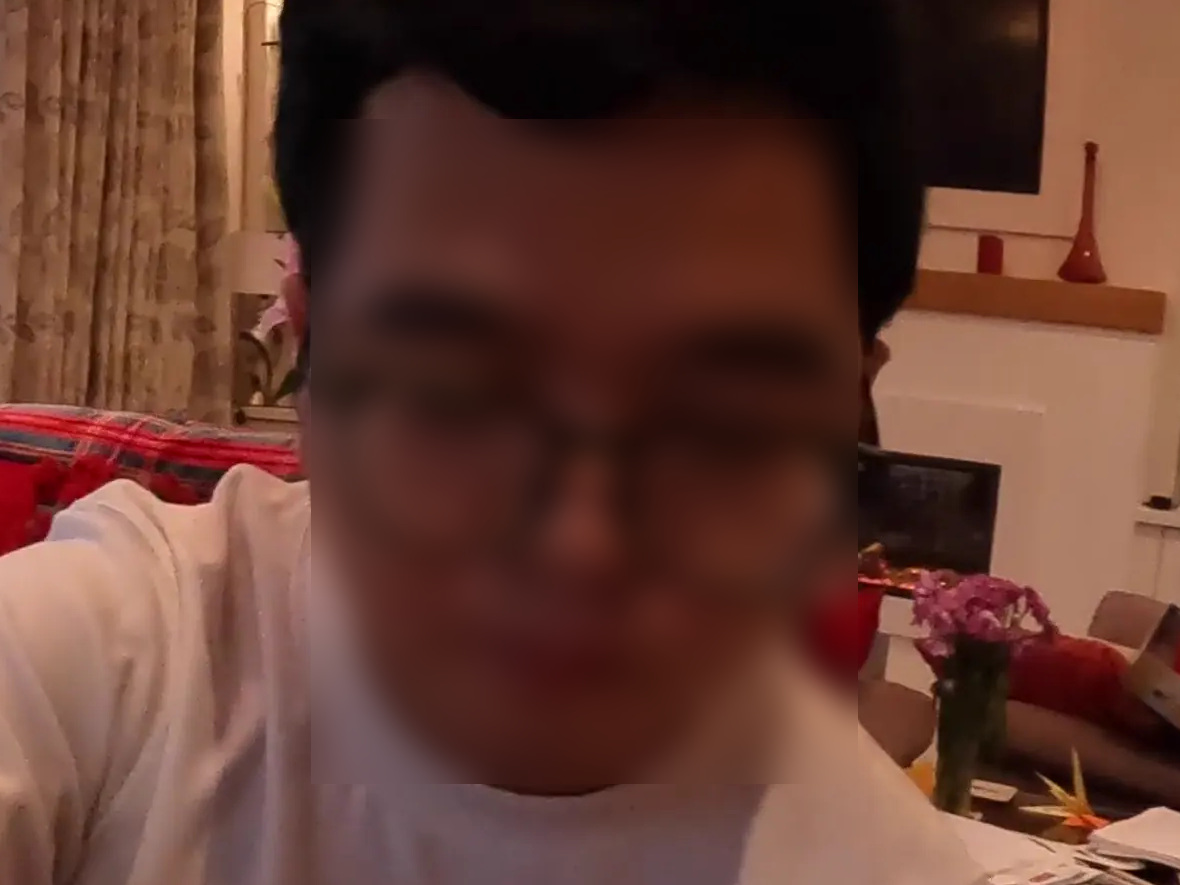
\includegraphics[trim=147 0 148 0,clip,width=.36\columnwidth]{images/rq2_castle_blur.jpg} &
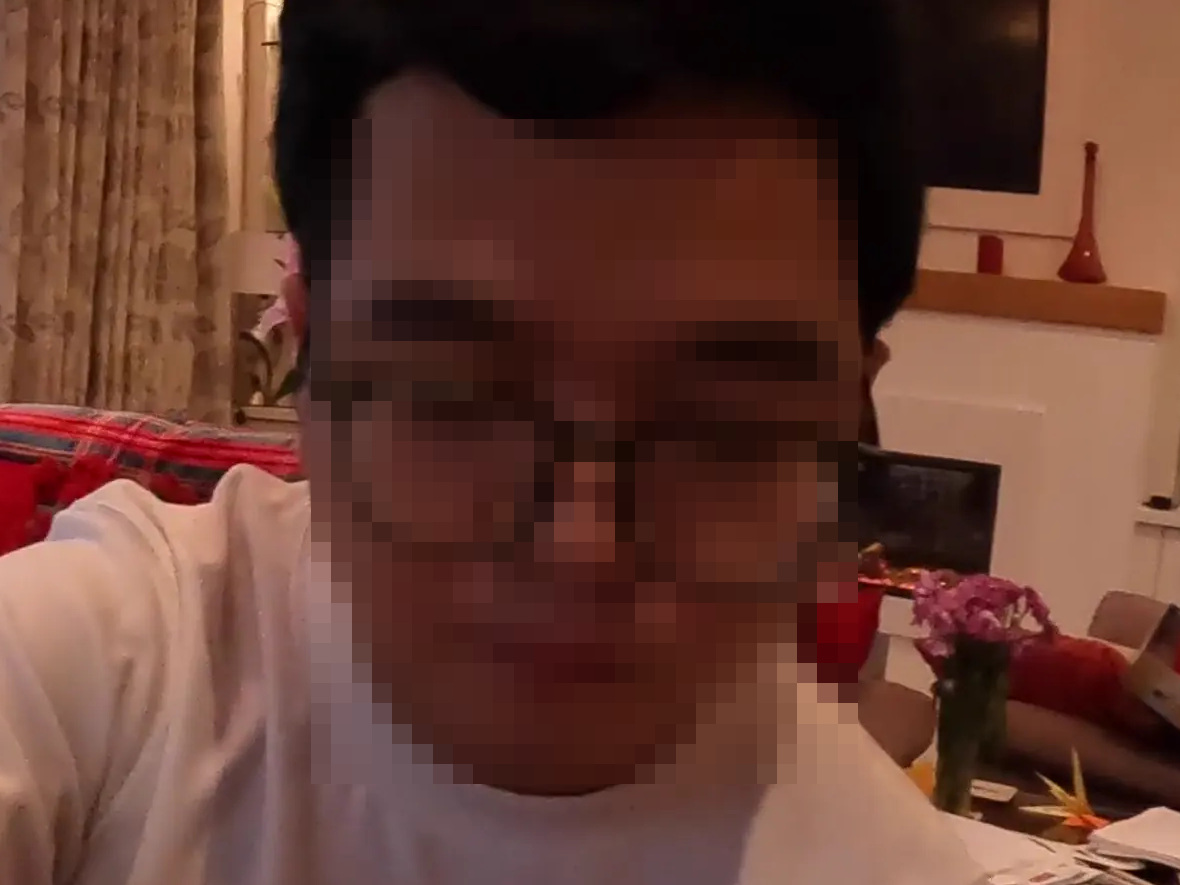
\includegraphics[trim=147 0 148 0,clip,width=.36\columnwidth]{images/rq2_castle_pixelate.jpg} \\
\scriptsize (a) Blur & \scriptsize (b) Pixelate \\
\multicolumn{2}{c}{\vspace{1pt}} \\
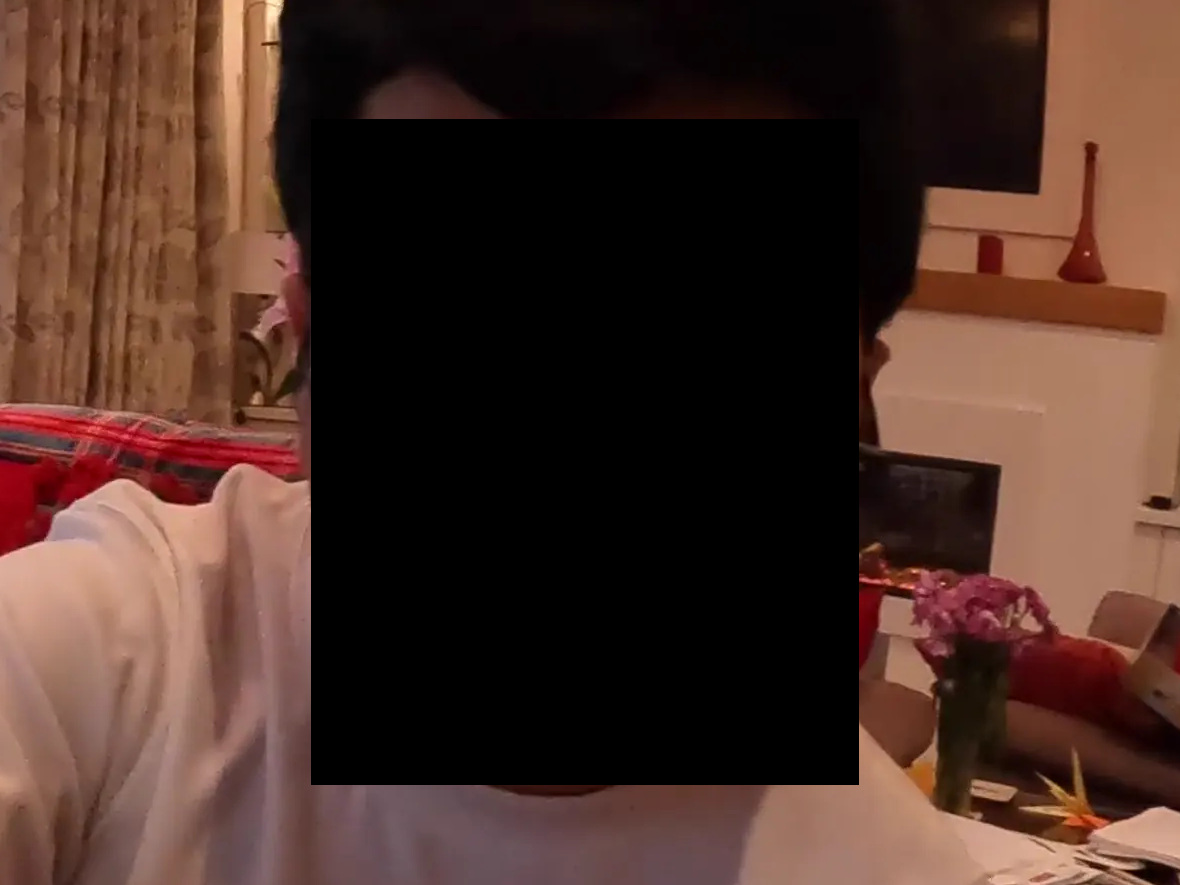
\includegraphics[trim=147 0 148 0,clip,width=.36\columnwidth]{images/rq2_castle_solid_mask.jpg} &
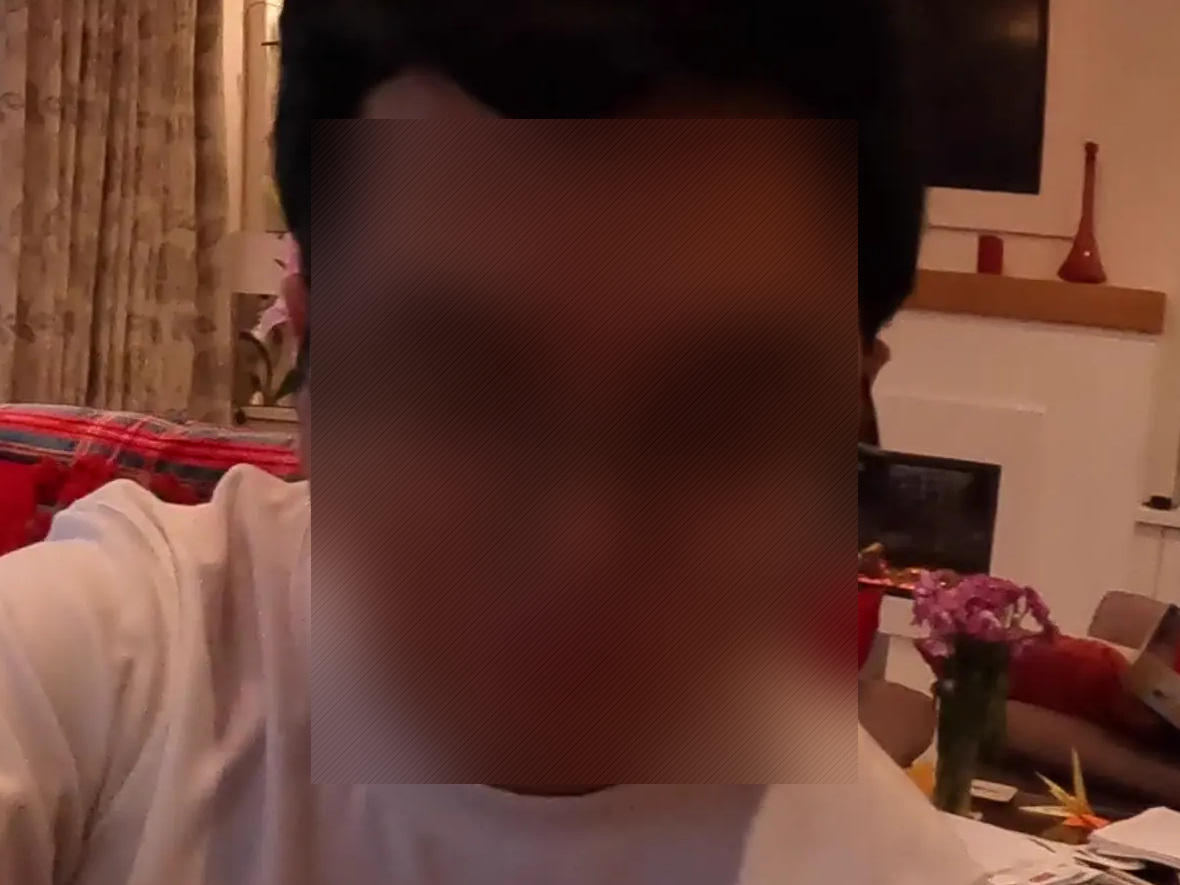
\includegraphics[trim=147 0 148 0,clip,width=.36\columnwidth]{images/rq2_castle_layered.jpg} \\
\scriptsize (c) Solid mask & \scriptsize (d) Layered
\end{tabular}
\caption{Deterministic protection outputs for the same reviewed face region
from a representative CASTLE frame \cite{rossetto2025castle}. The panel is
qualitative only; all numerical conclusions use the locked 500-image protocol.}
\label{fig:deterministic-comparison}
\end{figure}

\subsection{Metric and Visual-Review Boundaries}

SSIM and LPIPS are computed over the full frame, so their favourable values
partly reflect the small image area occupied by a face. They measure
preservation, not privacy. Re-identification is restricted to reviewed
face-positive frames using the denominators in Table~\ref{tab:rq2-deterministic}.
Equation~(\ref{eq:anon-privacy}) is applied per frame before aggregation. These
boundaries prevent full-frame similarity or missing attacker evidence from
being interpreted as privacy success.

Direct review checks residual identity, region coverage, collateral damage, and
conspicuous artefacts. It is not a blinded perceptual study. These non-synthetic
methods passed visual-safety eligibility, although protection still depends on
correct detection.

\subsection{Interim Answer to RQ2}

On the locked deterministic comparison, no method is universally best. Layered
protection achieved the highest observed composite score on the locked
protocol. Solid masking provided the strongest identity suppression,
pixelation the highest structural utility, and blur remained the stable
practical baseline. Layered combines $P=0.9808$ with more
utility than total masking; solid masking achieves the highest privacy component
but the lowest utility. Pixelation leaves substantially more identity evidence.
The atomic results explain why the score ordering alone is
insufficient: pixelation has the best SSIM and LPIPS but the weakest privacy,
whereas total masking produces the best AdaFace and ArcFace suppression at the
largest utility cost. Visual review remains decisive because metrics cannot
establish the absence of privacy leakage or unacceptable alteration.

The following analysis tests whether advanced methods improve these
deterministic reference points without introducing unacceptable failures or
visual distortion.

\clearpage

\begin{strip}
\centering
\refstepcounter{table}\label{tab:rq2-advanced}
{\footnotesize TABLE~\thetable\\
ADVANCED ANONYMISATION EVIDENCE AND FINAL METHOD ROLES\par}
\vspace{4pt}
\fontsize{7.2}{8.7}\selectfont
\setlength{\tabcolsep}{3.2pt}
\renewcommand{\arraystretch}{1.20}
\begin{tabular*}{\textwidth}{@{\extracolsep{\fill}}lrrrrrrr@{}}
\hline
\textbf{Method} & \textbf{Cov.} & \textbf{A/R $\downarrow$} &
\textbf{S/L} & \textbf{$t$ (s)} & \textbf{F} & \textbf{VQ} & \textbf{Role} \\
\hline
NF & 500/500 & .0532/.0837 & .9705/.0254 & 20.389 & 0 & n/q & RO \\
LD & 500/500 & .0250/.0360 & .9864/.0105 & 2.296 & 0 & 70/100 & RO \\
RP & 482/500 & .1476/.1768 & .9912/.0052 & 139.440 & 18 & n/q & RO \\
RD & 500/500 & .0039/.0016 & .9832/.0191 & .490 & 0 & 14/100 & RC \\
FA & 500/500 & .0016/.0016 & .9826/.0203 & 16.623 & 0 & 22/100 & RC \\
\hline
\end{tabular*}
\vspace{5pt}

\raggedright\footnotesize \textit{Notes:} NF: NullFace; LD: latent diffusion;
RP: Reverse Personalization; RD: RiDDLE; FA: FALCO. Cov.: successful/attempted;
A/R: AdaFace/ArcFace Re-ID; S/L: SSIM/LPIPS; $t$: mean seconds/frame; F:
failures; VQ: obvious artefacts/reviewed; RO: research only; RC: research
comparator. n/q: visually reviewed, not measured in the
fixed 100-output artefact audit. RP metrics: successful outputs.
\end{strip}

\begin{figure}[!t]
\centering
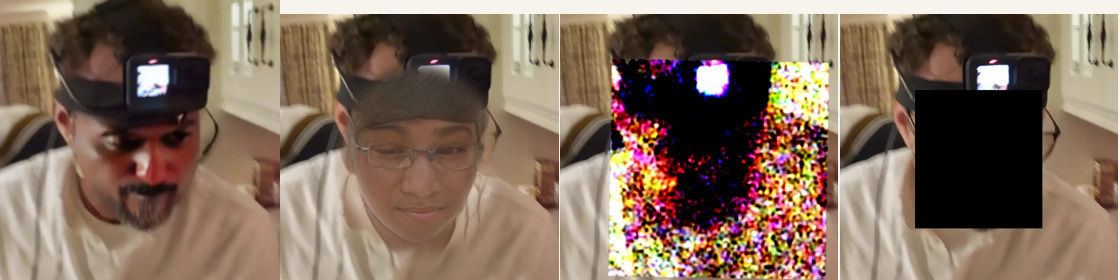
\includegraphics[width=\columnwidth]{images/rq2_advanced_comparison.jpg}
\vspace{1pt}

\scriptsize
\begin{tabular*}{\columnwidth}{@{\extracolsep{\fill}}cccc@{}}
(a) NullFace & (b) RiDDLE & (c) FAMS & (d) Solid mask
\end{tabular*}
\caption{The same reviewed CASTLE face region across three advanced methods and
a deterministic fallback \cite{rossetto2025castle}. NullFace alters facial
geometry, RiDDLE changes pose and gaze, FAMS introduces severe corruption, and
solid masking sacrifices utility predictably. The panel is qualitative only.}
\label{fig:advanced-failures}
\end{figure}

\subsection{Advanced Method Evaluation}

All methods retained the fixed manifest, reviewed regions, common attackers,
image metrics, runtime accounting, and failure-inclusive reporting from the
RQ2 protocol. NullFace used localised training-free synthesis, while the
low-step latent-diffusion branch used region-conditioned inpainting. Reverse
Personalization optimised a personalised latent representation
\cite{kung2026nullface,rombach2022ldm,kung2026reverse}. RiDDLE applied
invertible identity encryption, FALCO optimised a FaRL-guided latent code,
StyleID used a StyleGAN-based identity representation, and FAMS used
reference-conditioned diffusion
\cite{li2023riddle,barattin2023falco,le2023styleid,kung2025fams}.

Table~\ref{tab:rq2-advanced} reports the atomic results once. StyleID and FAMS
are excluded because neither completed the comparable 500-image metric
protocol; their pilot evidence is reported separately. The retained methods
have the following operational interpretation:
\begin{itemize}
\setlength{\itemsep}{1.5pt}
\setlength{\parskip}{0pt}
\setlength{\topsep}{2pt}
\item \textit{NullFace} completed the locked protocol and produced meaningful
identity suppression, but malformed facial geometry and slow execution blocked
default promotion.
\item \textit{Latent diffusion} preserved full-frame structure, but frequent
severe synthesis artefacts restricted it to research evidence.
\item \textit{Reverse Personalization} improved after targeted retry, yet
persistent failures, appearance drift, weak hard cases, and the slowest runtime
prevented operational use.
\item \textit{RiDDLE} achieved the highest observed advanced-method composite,
but pose and gaze changes and its recorded 80-GB accelerator boundary excluded
it from default routing.
\item \textit{FALCO} gave the strongest mean two-attacker identity suppression
among advanced methods, but visual failures and runtime limited it to a research
comparator.
\end{itemize}

StyleID and FAMS both failed to cross the final pilot visual-quality gate into
the locked 500-frame comparison. StyleID retained scale, placement, pose, and
compositing failures after its tuned 25-frame pilot. FAMS had broader
method-specific development evidence, but its repaired pilot and author-recipe
checks retained severe coloured corruption with the obtainable checkpoint.

\subsection{Why Metric-Only Selection Fails}

Full-frame SSIM and LPIPS are dominated by unchanged scene area, while low
Re-ID can reward any identity change, including an implausible synthetic face.
Direct review therefore tested facial geometry, gaze, pose, expression,
blending, and collateral alteration. It exposed altered gaze and expression,
warped geometry, hard compositing boundaries, unrealistic synthesis, and
synthetic insertion when a false-positive detector box was anonymised.
Figure~\ref{fig:advanced-failures} illustrates the mismatch directly.
This structured project review is independent of the numerical selection
score, but is not a blinded perceptual user study.

\subsection{Compute and Runtime Boundary}

Compute cost is part of method eligibility, not a deferred implementation
detail. Table~\ref{tab:rq2-advanced} reports measured mean end-to-end time;
the full NullFace run required 2~h 49~min 55~s, while Reverse Personalization
required 139.440~s per successful frame and still failed on 18 frames. RiDDLE
and FALCO were batch-evaluated on an 80-GB CUDA accelerator, peaking at 49.86
and 47.74~GiB respectively, so their timings are device-tied feasibility
evidence rather than laptop throughput claims. The later OAPR and App analysis
uses CUDA and VRAM tiers, measured same-device ETA, and safe method step-downs.

\subsection{Final Answer to RQ2}

No deterministic or advanced method was universally best on the reviewed
protocols. Advanced synthesis sometimes improved identity suppression or the
numerical privacy-utility trade-off, but visual acceptability, runtime,
coverage, and execution reliability changed the operational conclusion.
RiDDLE remains the strongest numerical research comparator and FALCO a
privacy-strong comparator, not default routes. Layered protection remains the
balanced default that passed the visual-safety gate, solid masking the
privacy-first fallback, and blur the stable practical baseline within the
evaluated framework. The next
analysis extends protection beyond faces to text and screens.

\clearpage

\section{RQ3: Integrated Visual Multimodal Privacy}
\label{sec:rq3}

Protecting faces alone leaves names, messages, documents, and displayed content
exposed. RQ3 therefore combines the established RQ1 face boxes with independently
reviewed text and screen evidence. CASTLE remains the experimental source, while
the question concerns comparable egocentric personal images more broadly
\cite{rossetto2025castle}.

\begin{strip}
\centering
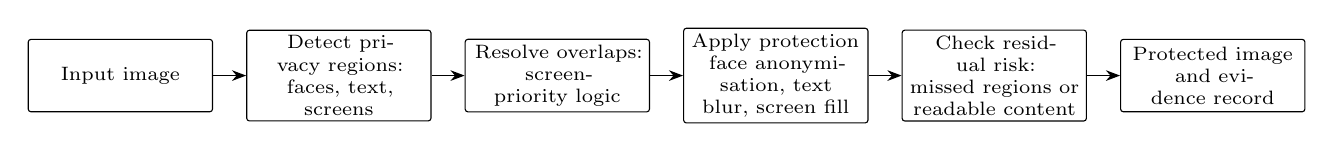
\begin{tikzpicture}[
  node distance=0.42cm,
  box/.style={draw, rounded corners=1pt, align=center, minimum height=0.92cm,
    text width=2.20cm, inner sep=2pt, font=\scriptsize},
  flow/.style={-{Stealth[length=1.8mm]}, line width=0.55pt}
]
\node[box] (input) {Input image};
\node[box, right=of input] (detect) {Detect privacy regions:\\faces, text, screens};
\node[box, right=of detect] (resolve) {Resolve overlaps:\\screen-priority logic};
\node[box, right=of resolve] (redact) {Apply protection\\face anonymisation, text blur, screen fill};
\node[box, right=of redact] (check) {Check residual risk:\\missed regions or readable content};
\node[box, right=of check] (output) {Protected image\\and evidence record};
\draw[flow] (input) -- (detect);
\draw[flow] (detect) -- (resolve);
\draw[flow] (resolve) -- (redact);
\draw[flow] (redact) -- (check);
\draw[flow] (check) -- (output);
\end{tikzpicture}
\vspace{1pt}

{\footnotesize Fig.~\refstepcounter{figure}\thefigure. RQ3 processing sequence.
The three privacy surfaces are detected together, overlaps are resolved,
protection is applied, and remaining risk is recorded.\label{fig:rq3-pipeline}\par}
\vspace{7pt}

\refstepcounter{table}\label{tab:rq3-heldout}
{\footnotesize TABLE~\thetable\\
HELD-OUT RQ3 COMPARISONS ON 75 REVIEWED IMAGES\par}
\vspace{4pt}
\fontsize{7.4}{8.9}\selectfont
\renewcommand{\arraystretch}{1.18}
\begin{minipage}[t]{0.485\textwidth}
\centering
\textit{A. Image-level privacy-risk presence}\par
\vspace{2pt}
\setlength{\tabcolsep}{2.5pt}
\begin{tabular*}{\linewidth}{@{\extracolsep{\fill}}lrrr@{}}
\hline
\textbf{Detected risk} & \textbf{Precision} & \textbf{Recall} & \textbf{F1} \\
\hline
Text present & .2766 & .8667 & .4194 \\
Screen present & .7917 & 1.0000 & .8837 \\
Text or screen present & .8333 & .9804 & .9009 \\
\hline
\end{tabular*}
\end{minipage}
\hfill
\begin{minipage}[t]{0.485\textwidth}
\centering
\textit{B. End-to-end redaction policies}\par
\vspace{2pt}
\setlength{\tabcolsep}{2.5pt}
\begin{tabular*}{\linewidth}{@{\extracolsep{\fill}}lrrrr@{}}
\hline
\textbf{Policy} & \textbf{$P_{\rm mm}$} & \textbf{$U$} &
\textbf{$t$ (s)} & \textbf{$S_{\rm mm-redact}$} \\
\hline
Adaptive policy & .8680 & .6634 & .667 & .8320 \\
Fixed blur/fill & .8680 & .6634 & .836 & .8319 \\
\hline
\end{tabular*}
\end{minipage}
\vspace{4pt}

\raggedright\footnotesize \textit{Note:} Each panel compares common measures on
the same 75 held-out images. In Panel B, $t$ is mean seconds/image. Region
localisation is separate; faces use RQ1 evidence.
\end{strip}

\subsection{Reviewed Protocol and Detection Stack}

The locked protocol contains 250 manually reviewed images, split into 175 for
development and 75 held out for evaluation. Its ground truth comprises 116 text
boxes and 139 screen boxes. Configuration and thresholds were selected only on
development evidence for the core detectors. The later completion campaigns
inspected retained held-out residuals and are therefore reported as post-hoc
hardening, not a fresh untouched test estimate. The 250-image surface does not
re-score faces; instead, the established RQ1 detector supplies face boxes to
the integrated pipeline.

CRAFT with the development-selected 4K recall settings generates text proposals
\cite{baek2019craft}. Screens are detected by the selected union of YOLO11 passes
at 640 and 1280 pixels. This multi-resolution evidence addresses the scale and
partial-view difficulty also observed in specialised egocentric screen work
\cite{li2026screen}. Screen regions take priority, so overlapping text proposals
are removed rather than redacted twice. If YOLO returns no screen, a dense
linked text cluster can complete a screen hypothesis. A strict landscape
bottom-edge phone rule is considered only when the screen path remains empty.
On the retained held-out split, the documented post-hoc hardening sequence
reduced screen-presence misses from $5\rightarrow1\rightarrow0$; loose
high-false-positive rules were rejected.

Presence variants are compared using the project-designed score
\begin{equation}
S_{\mathrm{mm-det}}=0.65R+0.25F_{1}+0.10P .
\label{eq:mm-det}
\end{equation}
Recall receives the greatest weight because a missed privacy-positive image can
leave content exposed. F1 and precision retain penalties for imbalance and
unnecessary redaction. The score selects methods within this project and does
not replace the atomic metrics or define a universal privacy measure.

\subsection{Redaction and Residual Evidence}

Six deterministic text and screen operator combinations were evaluated using
predicted, not oracle, boxes. Development selection routes predicted no-risk
images to copy-through, text-only risk to text blur, and screen-containing risk
to text blur plus screen fill. Each attempted image retains privacy, utility,
runtime, success, and residual-risk fields. The corresponding project score is
\begin{equation}
S_{\mathrm{mm-redact}}=0.50P_{\mathrm{mm}}+0.30U+0.10R_t+0.10S ,
\label{eq:mm-redact}
\end{equation}
where $P_{\mathrm{mm}}$ measures text suppression and screen obscuration, $U$
measures retained image utility, $R_t$ is constrained runtime suitability, and
$S$ records execution success. In the implementation,
$P_{\mathrm{text}}=0.70P_{\mathrm{OCR}}+0.30O_{\mathrm{text}}$, and
$P_{\mathrm{mm}}$ is the mean of the active ground-truth modality scores:
$P_{\mathrm{text}}$ for text and $O_{\mathrm{screen}}$ for screens. A frame
with neither annotated risk scores 1.0. These fixed project weights support
selection, not a general anonymisation formula.

\subsection{Held-Out Results and Failure Boundary}

Panel A of Table~\ref{tab:rq3-heldout} compares image-level presence directly.
Screen recall reached 1.0000; environmental lettering and textures reduced text
precision. Their union reached $P=0.8333$, $R=0.9804$, and $F1=0.9009$.
The separate region audit remained weaker: text achieved $P=0.0679$,
$R=0.7600$, and $F1=0.1246$; screens achieved $P=0.4576$, $R=0.6429$, and
$F1=0.5347$ at IoU 0.50, with area coverage 0.8543. Neither presence nor
coverage proves complete semantic removal.

Panel B compares end-to-end policies. Privacy and utility were equal after
rounding; adaptive routing was slightly faster and scored 0.8320 against
0.8319. The near-identical scores show that adaptive routing remained
competitive, but do not establish a meaningful numerical advantage. Residual
evidence records two text misses, no screen miss, six readable-text cases, one
insufficiently obscured screen, and 37 images with utility below 0.50. These
categories are non-exclusive. The low-overlap screen case and contextual cues
remain explicit limitations.

\subsection{Answer to RQ3}

RQ3 finds that joint face, text, and screen protection provides high-recall,
auditable visual multimodal risk reduction, while imperfect localisation and
semantic removal preclude a complete-anonymisation claim.

\clearpage

\section{RQ4: Objective-Aware Privacy Router}
\label{sec:rq4}

A single face-protection method cannot optimise identity suppression, retained
scene content, runtime, reliability, and visual quality for every egocentric
image. OAPR therefore treats selection as a constrained decision over frozen
RQ1--RQ3 evidence, not as an unconstrained user preference. The image condition
profile identifies supported operating conditions, while the requested
privacy objective and available compute determine which evidence is relevant.

\begin{strip}
\centering
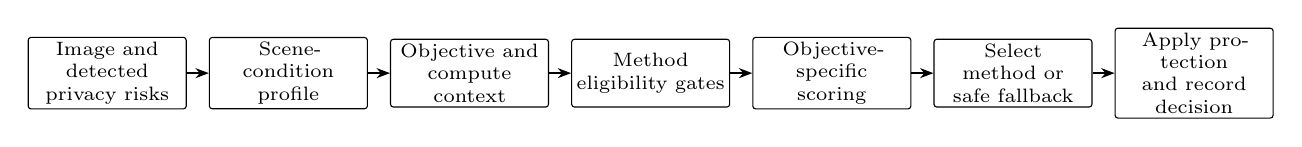
\begin{tikzpicture}[
  node distance=0.28cm,
  box/.style={draw, rounded corners=1pt, align=center, minimum height=0.86cm,
    text width=1.88cm, inner sep=1.8pt, font=\scriptsize},
  flow/.style={-{Stealth[length=1.7mm]}, line width=0.52pt}
]
\node[box] (input) {Image and detected\\privacy risks};
\node[box, right=of input] (profile) {Scene-condition\\profile};
\node[box, right=of profile] (context) {Objective and\\compute context};
\node[box, right=of context] (gate) {Method\\eligibility gates};
\node[box, right=of gate] (score) {Objective-specific\\scoring};
\node[box, right=of score] (select) {Select method or\\safe fallback};
\node[box, right=of select] (output) {Apply protection\\and record decision};
\draw[flow] (input) -- (profile);
\draw[flow] (profile) -- (context);
\draw[flow] (context) -- (gate);
\draw[flow] (gate) -- (score);
\draw[flow] (score) -- (select);
\draw[flow] (select) -- (output);
\end{tikzpicture}
\vspace{2pt}

{\footnotesize Fig.~\refstepcounter{figure}\thefigure. OAPR runtime decision
sequence. Scoring occurs only after evidence and resource gates; an unsupported
route terminates in deterministic protection rather than an unverified
advanced method.\label{fig:oapr-flow}\par}
\vspace{2pt}

\begin{minipage}[t]{0.485\textwidth}

\subsection{Eligibility Gates}

For method $m$ and image evidence $x$, the project gate is
\begin{equation}
G_m(x)=G_{\rm success}\wedge G_{\rm privacy}\wedge
G_{\rm quality}\wedge G_{\rm runtime}.
\label{eq:oapr-gate}
\end{equation}
$G_{\rm success}$ requires available, reliable execution; $G_{\rm privacy}$
enforces the objective's privacy floor; $G_{\rm quality}$ applies the direct
visual findings from RQ2; and $G_{\rm runtime}$ covers measured runtime and
compute feasibility. A candidate is eligible only if every required term is
true. Thus, a strong Re-ID result cannot promote RiDDLE, FALCO, or another
advanced method after it fails the visual or resource boundary.
An empty eligible set invokes the supported deterministic fallback. OAPR
records rejected methods and reasons, selected and applied actions, runtime,
fallback use, and execution failures for later audit.

\end{minipage}
\hfill
\begin{minipage}[t]{0.485\textwidth}

\subsection{Constrained Selection and Objectives}

Selection is restricted to the surviving set:
\begin{equation}
m^{*}(x)=\mathop{\rm arg\,max}_{m:\,G_m(x)=1}\;S_m(x),
\label{eq:oapr-select}
\end{equation}
where $S_m(x)$ combines objective-specific privacy, utility, runtime, and
success evidence. Equations~\ref{eq:oapr-gate} and~\ref{eq:oapr-select} are
project-designed rules, not universal formulas.

The materialised research comparison contains seven objective identifiers:
privacy first, utility priority, utility under a privacy floor, runtime aware,
compute-profile adaptive, failure avoidance, and multimodal risk. Table
\ref{tab:oapr-materialised} compares their actual 500-image outputs with fixed
references on one common metric surface. Four objectives are grouped because
they produced identical routed images and metrics, not because their stated
purposes are interchangeable.
\end{minipage}

\vspace{3pt}

\centering
\refstepcounter{table}\label{tab:oapr-materialised}
{\footnotesize TABLE~\thetable\\
FIXED REFERENCES AND MATERIALISED OAPR OUTPUTS ON THE LOCKED 500-IMAGE PROTOCOL\par}
\vspace{2pt}
\fontsize{7.1}{8.55}\selectfont
\renewcommand{\arraystretch}{1.17}
\setlength{\tabcolsep}{3.2pt}
\begin{tabular*}{\textwidth}{@{\extracolsep{\fill}}p{3.25cm}p{3.30cm}rrrrrp{2.55cm}@{}}
\hline
\textbf{Objective or policy} & \textbf{Applied output} &
\textbf{SSIM$\uparrow$} & \textbf{LPIPS$\downarrow$} &
\textbf{Ada$\downarrow$} & \textbf{Arc$\downarrow$} &
\textbf{Success} & \textbf{Interpretation} \\
\hline
\multicolumn{8}{l}{\textit{A. Fixed reference policies}} \\
Fixed blur & Fixed blur policy, all frames & .9929 & .0080 & .0550 & .1158 & 500/500 & Balanced baseline \\
Fixed solid mask & Fixed mask policy, all frames & .9775 & .0195 & .0005 & .0006 & 500/500 & Privacy anchor \\
Fixed layered & Fixed blur/downscale/noise policy & .9893 & .0098 & .0136 & .0372 & 500/500 & Visual-safe default \\
\multicolumn{8}{l}{\textit{B. OAPR objective modes, actual routed outputs}} \\
Privacy first & 354 mask, 146 copy & .9793 & .0186 & .0008 & .0008 & 500/500 & Strongest suppression \\
Failure avoidance & 333 layered, 21 blur, 146 copy & .9911 & .0090 & .0102 & .0281 & 500/500 & Reliability-led balance \\
Runtime aware & 275 layered, 79 blur, 146 copy & .9912 & .0088 & .0164 & .0344 & 500/500 & Runtime-sensitive mix \\
Utility priority / privacy floor / compute adaptive / multimodal risk & 354 blur, 146 copy & .9915 & .0088 & .0258 & .0555 & 500/500 & Identical measured output \\
\hline
\end{tabular*}
\vspace{3pt}

\raggedright\footnotesize \textit{Note:} Panel A repeats the fixed all-frame
policies in Table~\ref{tab:rq2-deterministic}. Routed rows combine protection
with unchanged no-action outputs. Copy denotes an unchanged output where no
face-protection action is eligible. Ada and Arc are AdaFace and ArcFace Re-ID
rates. All OAPR rows are materialised outputs, not simulations. Across the seven
modes, runtime ranged from 0.395 to 0.431 s/image.

\vspace{3pt}
\begin{minipage}[t]{0.485\textwidth}

\subsection{Interpretation}

Privacy-first routing approached the fixed mask's near-zero Re-ID rate, but retained
its visible utility cost. Failure avoidance preserved substantially more image
similarity while improving identity suppression over blur. Runtime-aware routing
occupied an intermediate operating point. The utility-led group remained close
to blur because blur was its strongest eligible fallback. Across all seven
modes, mean materialisation runtime ranged from 0.395 to 0.431 s/image and every
mode completed 500/500 outputs without a policy failure. These observed
trade-offs do not establish global dominance over blur or statistical
superiority between neighbouring scores.

The strengthened visual gate fixed the balanced scientific route at 286
layered outputs, 81 solid masks, and 133 reviewed no-face copy-through frames.
The four grouped objectives retain different intentions; their identical
outputs reflect the eligible methods on this protocol rather than equivalent
objective definitions.
\end{minipage}
\hfill
\begin{minipage}[t]{0.485\textwidth}

\subsection{Visual-Safe Decision and Answer}

It completed 500/500 routes with no generative selections, zero failures, and a
recorded balanced-objective score of 0.9562. Table~\ref{tab:oapr-materialised}
compares fixed policies with earlier objective-mode routes on the locked
face-box surface. The hardened result additionally applies detector-informed
safety gates, so its distribution and composite score are reported separately.
The gate overrode 13 candidate no-action decisions when high-confidence face
evidence remained, reducing 146 initial copy routes to 133 safe copies. These
extra protection actions are a utility cost, not execution failures. This
explains why direct visual and safety eligibility can supersede an attractive
metric-only route.

RQ4 therefore finds that OAPR supports auditable, condition-aware and
objective-aware selection across the evaluated heterogeneous egocentric
conditions. Its contribution is explicit objective selection, exclusion of
unsupported or visually unsafe candidates, adaptation to compute and failure
evidence, deterministic fallback, and a reviewable decision record, rather than
universal metric dominance or complete anonymisation.
\end{minipage}
\end{strip}
\mbox{}

\clearpage

\section{Research Demonstrator}
\label{sec:demonstrator}

The implemented App converts the research into an accessible end-to-end privacy
workflow. It brings compute-aware planning, face, text, and screen detection,
editable review, protection, previews, and audit reporting into one interface.
The result is a practical demonstrator of how the verified methods and OAPR
evidence can guide real image protection without requiring the operator to
understand each model or metric.

\begin{strip}
\centering
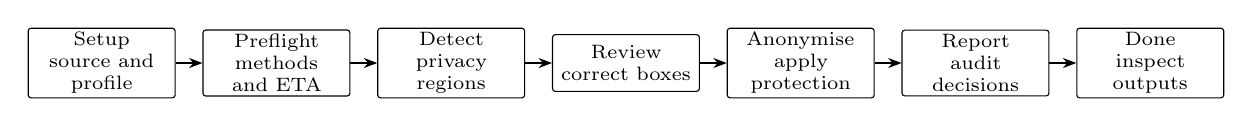
\begin{tikzpicture}[
  node distance=0.34cm,
  box/.style={draw, rounded corners=1pt, align=center, minimum height=0.72cm,
    text width=1.76cm, inner sep=1.5pt, font=\scriptsize},
  flow/.style={-{Stealth[length=1.7mm]}, line width=0.52pt}
]
\node[box] (setup) {Setup\\source and profile};
\node[box, right=of setup] (preflight) {Preflight\\methods and ETA};
\node[box, right=of preflight] (detect) {Detect\\privacy regions};
\node[box, right=of detect] (review) {Review\\correct boxes};
\node[box, right=of review] (protect) {Anonymise\\apply protection};
\node[box, right=of protect] (report) {Report\\audit decisions};
\node[box, right=of report] (done) {Done\\inspect outputs};
\draw[flow] (setup) -- (preflight);
\draw[flow] (preflight) -- (detect);
\draw[flow] (detect) -- (review);
\draw[flow] (review) -- (protect);
\draw[flow] (protect) -- (report);
\draw[flow] (report) -- (done);
\end{tikzpicture}
\vspace{2pt}

{\footnotesize Fig.~\refstepcounter{figure}\thefigure. Operator journey through
the App demonstrator. Review is optional, but the remaining stage order is
enforced so that method intent and execution records stay aligned.
\label{fig:app-journey}\par}
\vspace{3pt}

\begin{minipage}[t]{0.485\textwidth}
\centering
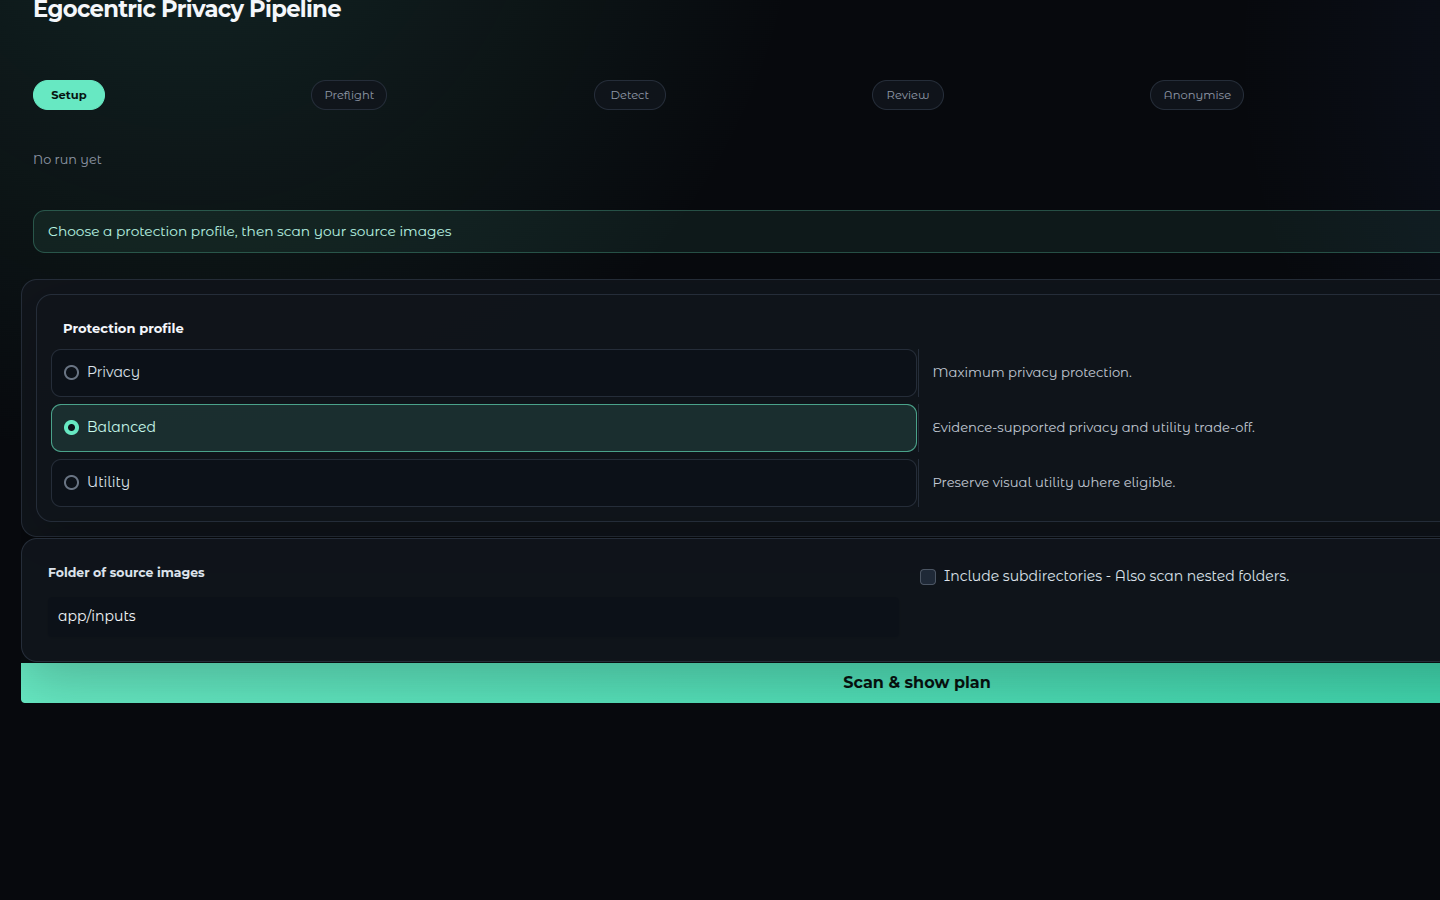
\includegraphics[width=0.96\linewidth]{images/app_setup_column.png}
\vspace{1pt}

{\footnotesize (a) Setup selects the source and the intended Privacy, Balanced,
or Utility profile before any models are loaded.\par}
\raggedright
\small

\subsection{Guided Preflight}

Setup accepts an image folder and a Privacy, Balanced, or Utility profile.
Preflight scans the workload, summarises detected risks, presents the available
processing stages and method choices, and estimates duration before heavy models load. OAPR
evidence informs the proposed methods, while detected CUDA availability and
memory determine their compute-fit status. The operator can accept the complete
plan or inspect and change any stage.

\subsection{Compute-Aware Protection}

After confirmation, the App streams face and visual multimodal detection
progress. It selects an evidence-backed detector tier for the available
hardware, while low-cost deterministic protection keeps anonymisation practical
on lower-compute systems. More capable accelerators can expose the advanced
research methods through the same interface. This tiered design allows one
workflow to scale from portable hardware to high-memory GPU execution.

\subsection{Reviewer Control and Outputs}

The reviewer separates face, screen, and text layers and permits boxes to be
added, moved, resized, or deleted before protection. Completion then creates
protected images, side-by-side previews, per-image decisions, runtime records,
and a readable report. Selected and applied methods, including any safe
fallback, remain visible, so a reviewer can follow the complete run from user
intent to the final pixel operation.
\end{minipage}
\hfill
\begin{minipage}[t]{0.485\textwidth}
\centering
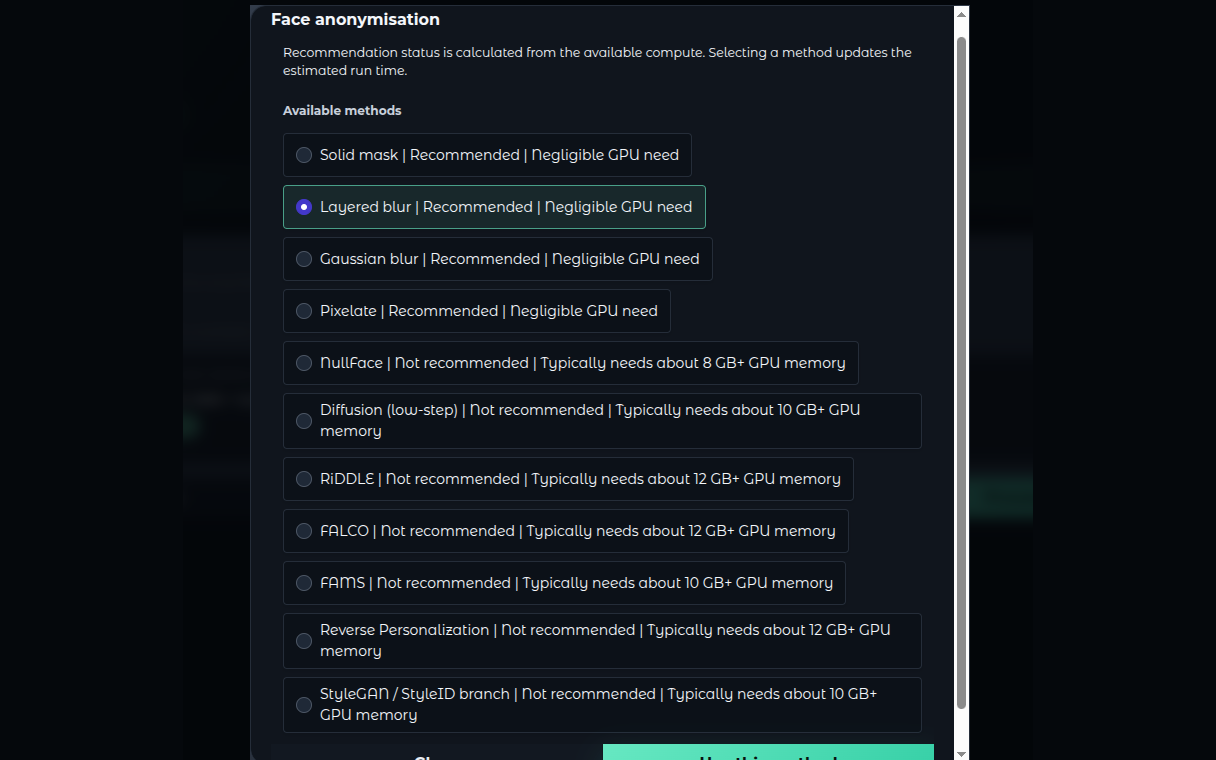
\includegraphics[width=0.96\linewidth]{images/app_anonymisation_selector_column.png}
\vspace{1pt}

{\footnotesize (b) The anonymisation selector compares deterministic and
advanced methods and shows their compute requirements before execution.\par}
\raggedright
\small

\subsection{Evidence-Backed Potential}

The App operationalises the detector roles, visual-safety decisions, method
eligibility, runtime boundaries, and fallbacks established by the OAPR evidence.
Recommendations therefore reflect experimental privacy, utility, reliability,
visual-quality, and compute findings rather than model popularity alone. The
selector makes those choices understandable by showing which methods fit the
available hardware before execution begins.

\subsection{Demonstration Value}

The demonstrator makes the full framework tangible in one session: it discovers
the workload, recommends a feasible plan, exposes alternative methods, supports
human correction, protects three privacy surfaces, and produces inspectable
outputs and records. Progress indicators and stage navigation make long jobs
understandable, while the modular backends allow new detectors and anonymisers
to be added without redesigning the operator journey.

\subsection{Limits and Extension}

The measured values remain tied to the reviewed protocols, tested methods, and
hardware, and residual contextual cues can remain after regional protection.
Broader egocentric collections, user studies, and additional devices should be
evaluated next. The App's tiered execution, editable review, safe fallbacks, and
audit trail provide a strong platform for that extension.
\end{minipage}
\end{strip}
\mbox{}

\clearpage

\begin{strip}
\begin{minipage}[t]{0.485\textwidth}
\small
\linespread{1.035}\selectfont
\setlength{\parskip}{3.5pt}
\section{Conclusion}

This study developed and evaluated an evidence-bounded visual multimodal
privacy framework for egocentric personal images. Rather than treating face
anonymisation, text redaction, screen protection, visual quality, runtime, and
failure handling as separate concerns, the framework connects them through
reviewed protocols and an objective-aware selection layer.

RQ1 showed that detector choice depends on the operating objective. The
hardened random-forest policy provided the strongest balanced operating point,
with $P=0.9319$, $R=0.9129$, $F1=0.9223$, and a project score of 0.9172, while
precision-led and recall-led alternatives retained useful roles.

RQ2 found no universal anonymiser. Advanced methods could improve numerical
identity suppression, but execution cost and direct visual artefacts changed
their final eligibility. Layered protection remained the balanced visually safe
default, with solid masking and blur providing predictable privacy-first and
practical fallbacks.

RQ3 extended protection to faces, text, and screens within one RGB-image
policy. Combined-risk presence detection reached 0.9804 recall on the held-out
split, while region-level and residual-readability audits exposed the remaining
localisation and semantic boundary.

RQ4 showed that OAPR can convert these heterogeneous findings into inspectable
decisions. Its hardened balanced route completed all 500 outputs with zero
execution failures and a recorded score of 0.9562, while safety gates replaced
13 candidate no-action decisions with protection.

The App demonstrates the practical value of this integration. It offers guided
preflight planning, compute-aware recommendations, editable multimodal review,
fast deterministic operation on modest hardware, advanced options when compute
permits, and traceable protected outputs. The principal contribution is thus
not a claim that one model solves every privacy condition, but a reproducible
way to combine evidence, visual review, compute constraints, and safe fallbacks.
Future work should validate the framework on further egocentric collections,
additional hardware, video sequences, and broader reviewer studies.

\section*{Declaration of Generative AI Use}

Google Gemini was used during the project for coding assistance within Google
Colab, including code suggestions and debugging support. Gemini was also used
during report preparation to assist with language refinement, LaTeX code, and
document formatting. The project README files were generated with Gemini.
Its outputs were iteratively reviewed, corrected, and accepted or rejected by
the authors.

Gemini did not replace the authors' implementation, manual annotation,
experimental execution, visual review, result interpretation, or final
judgement. All reported values and claims were checked against the project
evidence by the authors. No other generative AI model was used. The authors take
responsibility for the submitted work and confirm that they have conformed to
the applicable regulations on the use and declaration of Generative AI.
\end{minipage}
\hfill
\begin{minipage}[t]{0.485\textwidth}
\section*{References}
\renewcommand*{\bibfont}{\fontsize{6.5}{7.0}\selectfont}
\setlength{\bibitemsep}{0.35pt}
\setlength{\biblabelsep}{2.5pt}
\printbibliography[heading=none]
\end{minipage}
\end{strip}
\mbox{}

\end{document}
